
\section{Use Cases and Evaluation}

As of today, we have mostly evaluated the iFLUX from a developer's point of view. We have looked at the following questions: how easy is it to grasp the programming model? How easy is it to create a new service or to expose a legacy service through iFLUX APIs? How easy is it to build an application by applying the programming model? To answer these questions, we have worked with various teams to develop both components and applications. These teams had no prior knowledge about iFLUX before starting the exercise. In all cases, we saw that it was easy and quick both to implement iFLUX APIs in existing components and to design end-to-end workflows.

\begin{figure*}
\centering
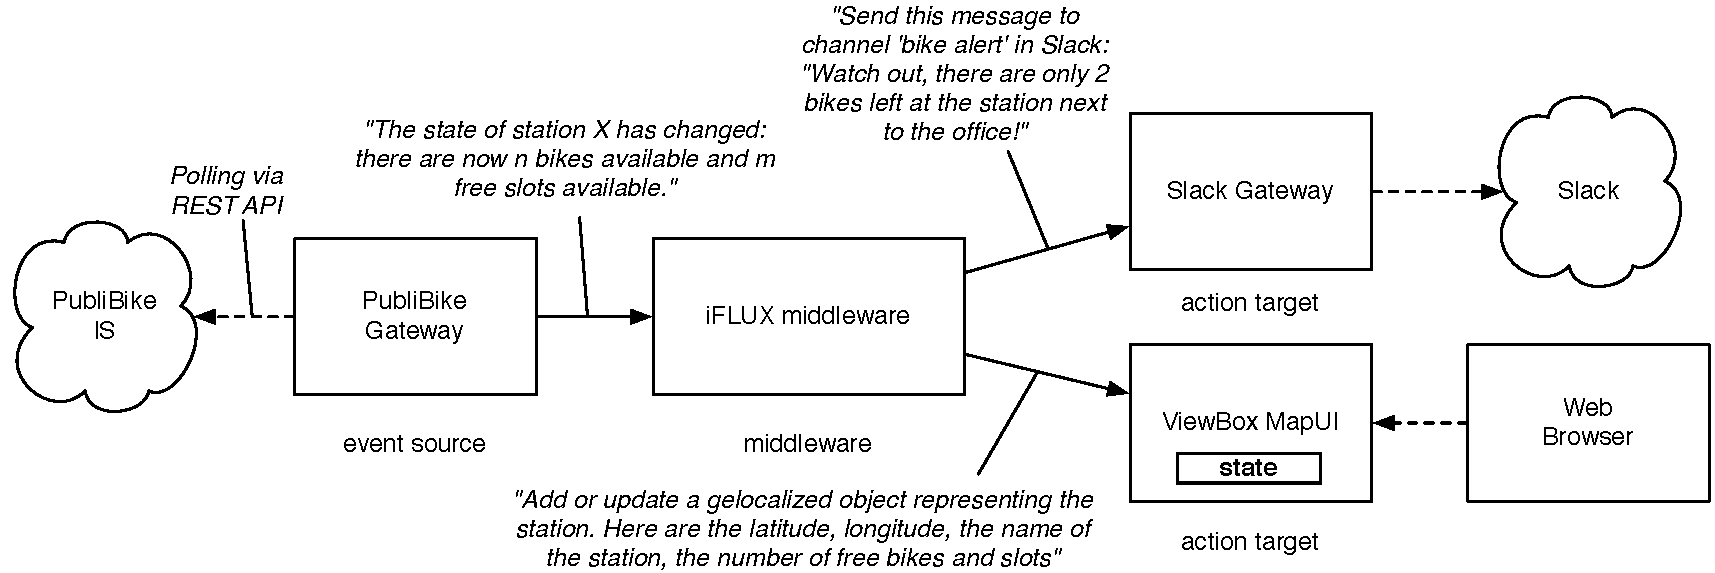
\includegraphics[width=0.7\textwidth]{figures/publibike.pdf}
\caption{The PubliBike application, with one event source and two action targets}
\label{fig:publibike}
\end{figure*}

\begin{figure*}
\centering
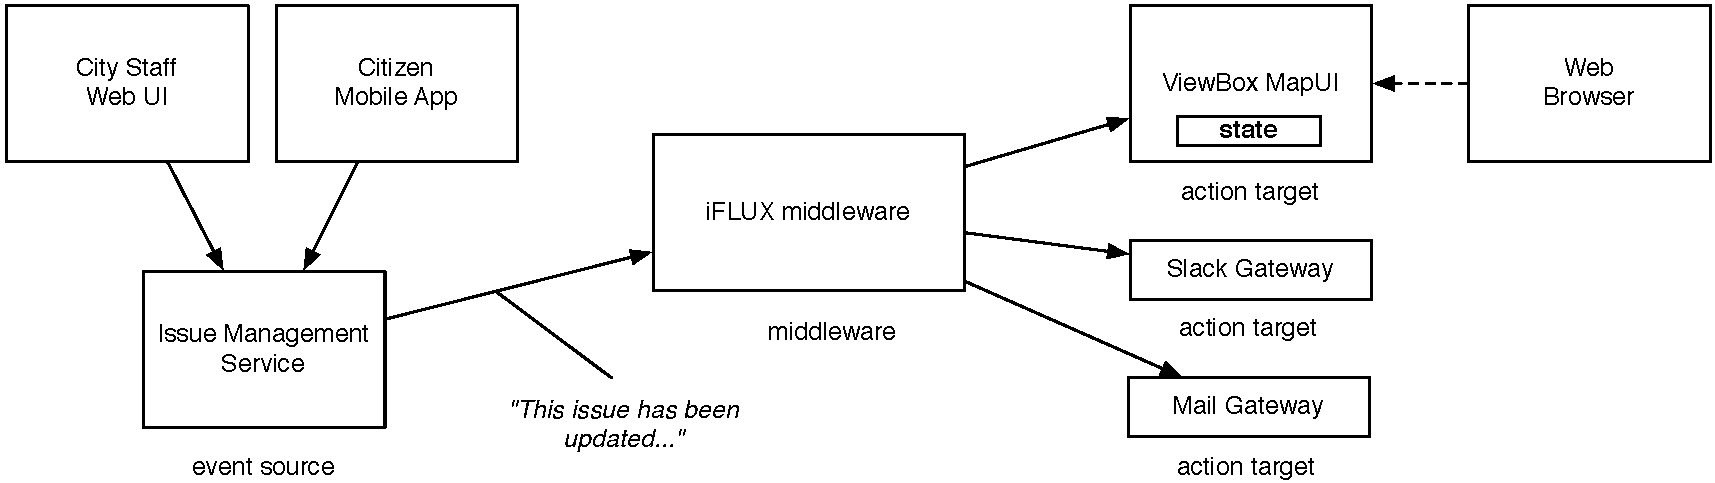
\includegraphics[width=0.7\textwidth]{figures/citizen}
\caption{The Citizen Engagement application, with one event source and three action targets}
\label{fig:citizen}
\end{figure*}

%\begin{figure*}
%\centering
%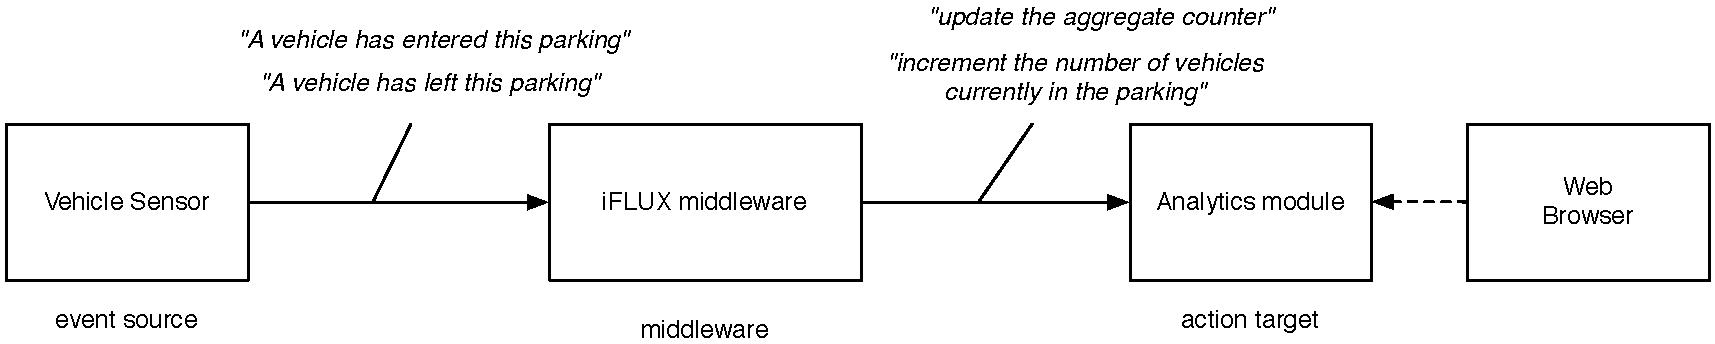
\includegraphics[width=0.9\textwidth]{figures/paleo}
%\caption{The Paléo Festival application, with one event source and one action target}
%\label{fig:paleo}
%\end{figure*}

%\begin{figure*}
%\centering
%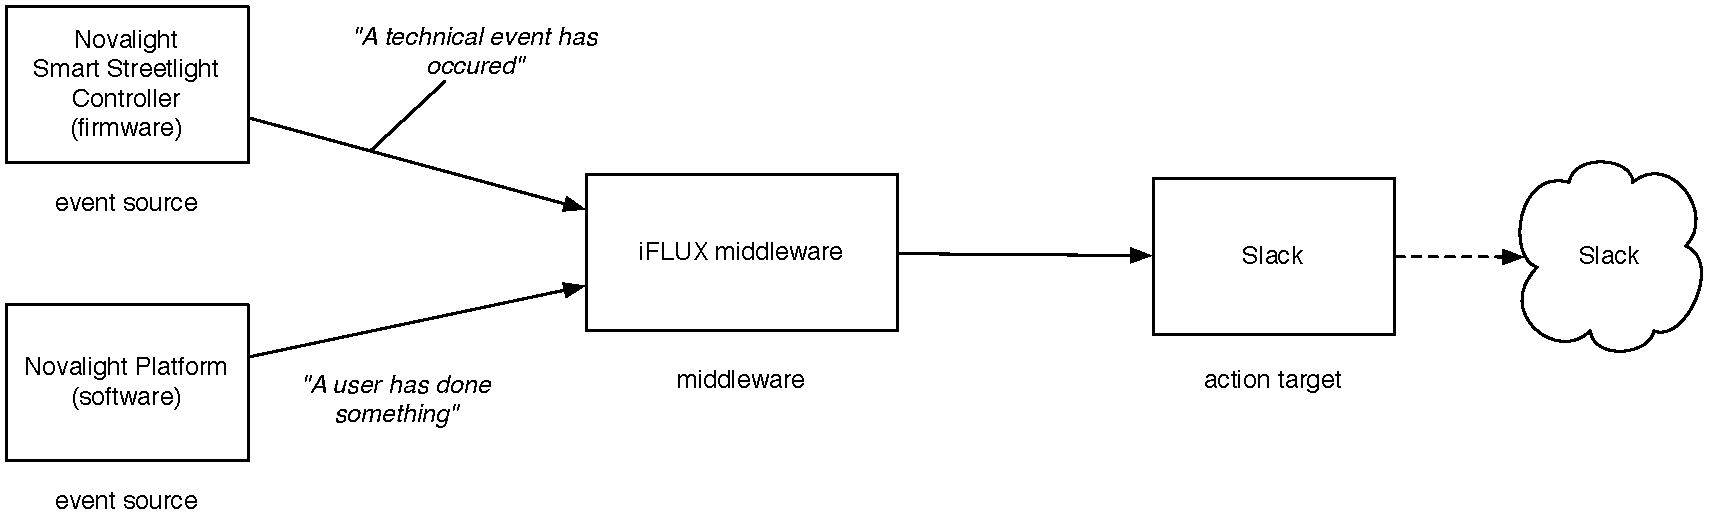
\includegraphics[width=0.9\textwidth]{figures/awareness}
%\caption{The Awareness @ Novaccess application, with two event sources and one action target}
%\label{fig:paleo}
%\end{figure*}


\subsection{PubliBike}

Like in many other countries, bike sharing stations are increasingly deployed in swiss cities (see Figure \ref{fig:publibikeStation}). Customers need to acquire a smart card, with which they can unlock a bike at a station. They also use the smart card when they later return the bike. The bike stations are connected to a nation-wide information system, named PubliBike. PubliBike makes it possible to know the number of available bikes and free slots at every station, in realtime. The data can be accessed via a REST API: the returned JSON payload contains the current state of all stations.

\begin{figure}[H]
\centering
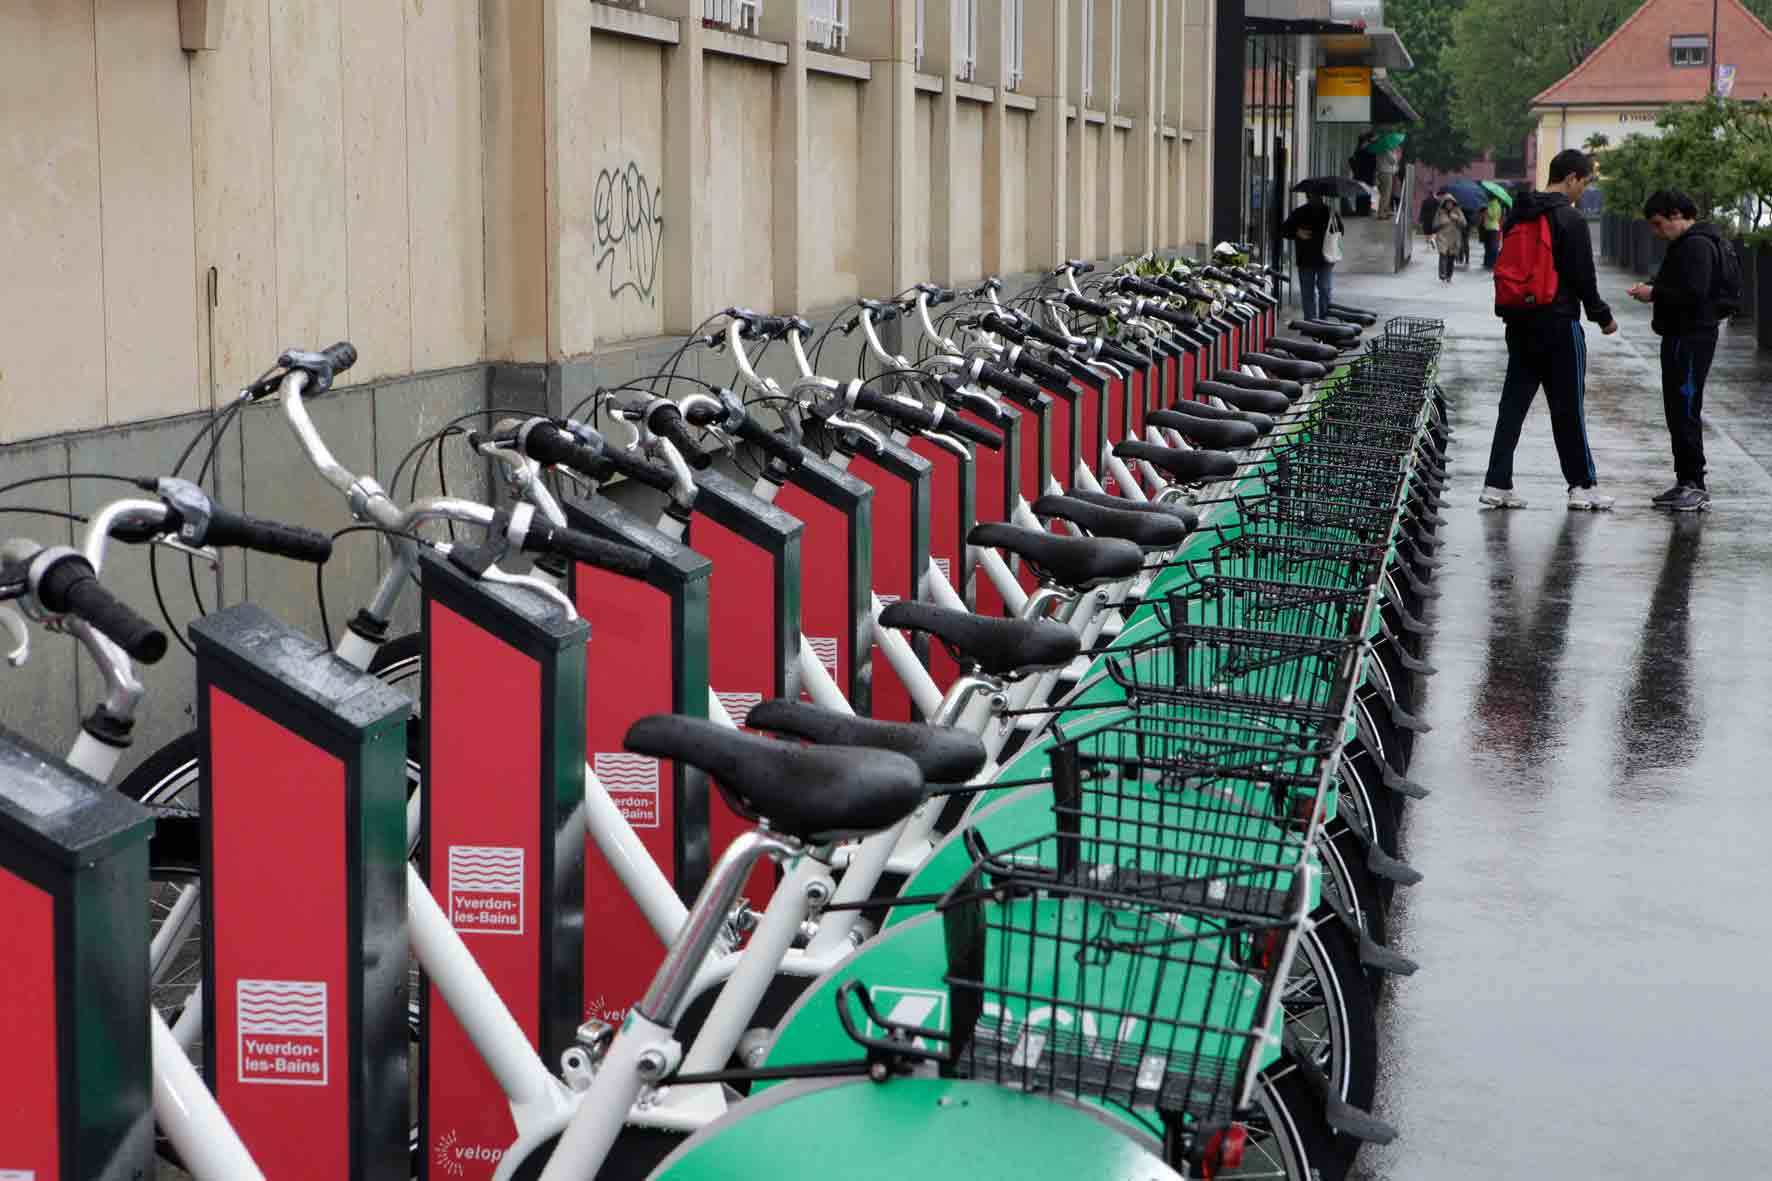
\includegraphics[width=0.85\columnwidth]{figures/publibikephoto2.jpg}
\caption{A bike station in Yverdon-les-Bains}
\label{fig:publibikeStation}
\end{figure}

\begin{figure}[H]
\centering
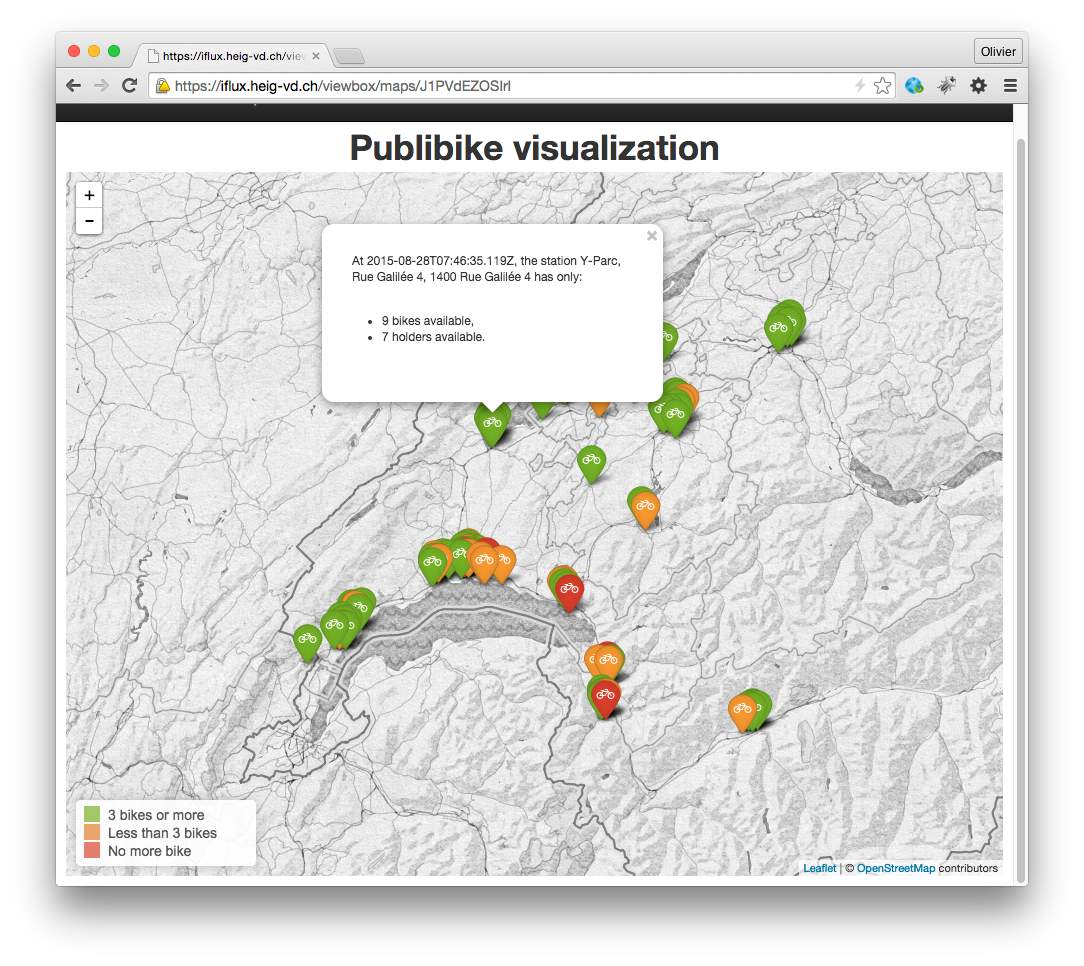
\includegraphics[width=0.75\columnwidth]{figures/publibike-viewbox.png}
\caption{Bike stations displayed by an action target}
\label{fig:publibikeMap}
\end{figure}


As illustrated in Figure \ref{fig:publibike}, we have implemented one \emph{event source} and two \emph{action targets} and we have defined rules in order to react to the activity monitored within the PubliBike system. These components are described in the following paragraphs.

\subsubsection{Tracking bike arrival and departure: the PubliBike Event Source}
Integrating PubliBike into the iFLUX ecosystem has first been achieved by defining a new \emph{event source} and by specifying the type of events produced by this source. Note that when doing this, we did not need to think about how the information would be used. It could be used to trigger alerts, to create visual representations, to compute statistics. As developers of the \emph{event source}, this is not something that we had to worry about (decoupling). We could have decided to define one \emph{event source} for every bike station, but instead we have preferred to define a single \emph{event source}: the PubliBike gateway, which is responsible for polling data via the PubliBike API and to detect state changes. In this scenario, while there are sensors and communication modules embedded in the physical stations, the iFLUX \emph{event source} is purely implemented in a software daemon running in the cloud. With the PubliBike \emph{event source} deployed, iFLUX receives an incoming stream of events, where every event represents a state change at a given station (i.e. either a bike has arrived or left). In addition to a timestamp, the events contain the following properties: the identifier, name and geographic coordinates of the station, the number of available bikes and the number of free slots. 

\subsubsection{Notifying users: the Slack action target}
Someone who uses the bike sharing service to commute from the office to the train station might be interested to be notified if the number of available bikes close to the office falls below a certain threshold. This person might also be interested to receive an alert if the number of free slots at the station falls below a threshold. To implement this use case, the user needs an iFLUX \emph{action target} that provides a bridge to a notification system (SMS, e-mail, etc.). To illustrate the idea, we have implemented an action target that makes it possible to send a notification in the Slack instant messaging platform \cite{slack}. The payloads sent to the action target via the REST API contain the message and the name of the channel where to post it. 

This allows the user to define an iFLUX rule, which states that \emph{\textbf{IF} an event is received from the PubliBike event source AND the event property `stationId' of the event is the one of the station close to my office AND if the event property `numberOfAvailableBike' is less than 3 \textbf{THEN} send an action to the Slack action target, with the property `channel' set to `bike alerts' and the property `message' set to `WARNING: there are not many bikes left at the station!'}. 

\subsubsection{Map visualization: the ViewBox action target}
Another idea for using the data produced by the PubliBike event source was to create a visual representation, where the current state of every bike station is shown on a geographical map (see Figure \ref{fig:publibikeMap}). This use case is interesting, because it raises the question about how to deal with application state given that iFLUX rules are stateless.

We have implemented an \emph{action target} that we have named the \emph{ViewBox action target}. Note that while it can be used in conjunction with the \emph{PubliBike event source}, it is generic and can be used with other types of \emph{event sources} (for instance, it has been used in the citizen engagement application described later). Essentially, the \emph{ViewBox action target} is responsible for managing application state, which is defined by a collection of geolocalized objects, which can have arbitrary properties attached to them. It accepts action payloads with the following properties: the unique identifier of a geolocalized object, the current latitude and longitude and a list of application specific values (in the case of PubliBike, the name of the station and the number of available bikes and slots). When it receives an action via the REST endpoint, it creates or updates a geolocalized object with the property values in the payload. The \emph{action target} provides its own API (outside the scope of iFLUX), so that web browsers can fetch annotated maps. 

After deploying the \emph{Viewbox action target}, we were able to configure a rule so that whenever an event was received from the \emph{PubliBike event source}, an action would be sent to the \emph{ViewBox action target} to update the corresponding geolocalized object.


%\FloatBarrier



\subsection{Citizen Engagement}

After a few months of work on iFLUX, we used the platform in a two-weeks undergraduate course dedicated to end-to-end mobile services. The course is project-oriented and every year, we use an application domain to provide some context to the students. This year, we explained that software platforms are increasingly deployed, so that citizen can report issues to city authorities \cite{patel2015guide,offenhuber2014infrastructure}. Users can report broken street lights, graffitis, dangerous areas, etc. The students were asked to design a system with two components. Firstly, they had to implement a simple issue tracking system and to expose their domain model via a RESTful API. Secondly, they had to implement a mobile app that would be provided to citizen, so that they could easily report issues and follow their resolution process.

The Citizen Engagement back-end was then transformed into an iFLUX \emph{event source}. This was done by emitting an event whenever the state of an issue would change (created, acknowledged, in progress, resolved, etc.). Special properties were added to the event (e.g. to attach comments to state transitions). Again, since emitting an iFLUX event is not more complicated than issuing a POST request, the integration was trivial. 
%As illustrated in Figure \ref{fig:citizenEngagement}, 
We were then able to combine the new \emph{event source} with existing \emph{action targets}. It was really easy to implement a workflow to notify city staff about new issues, either via Slack or via email. It was also very easy to create a map to visualize the issue with the \emph{Viewbox action target} described before. Figure \ref{fig:citizen} shows the end-to-end workflow in iFLUX. Several rules have been added to trigger behavior in the action targets whenever an issue is updated.

%\begin{figure}
%\centering
%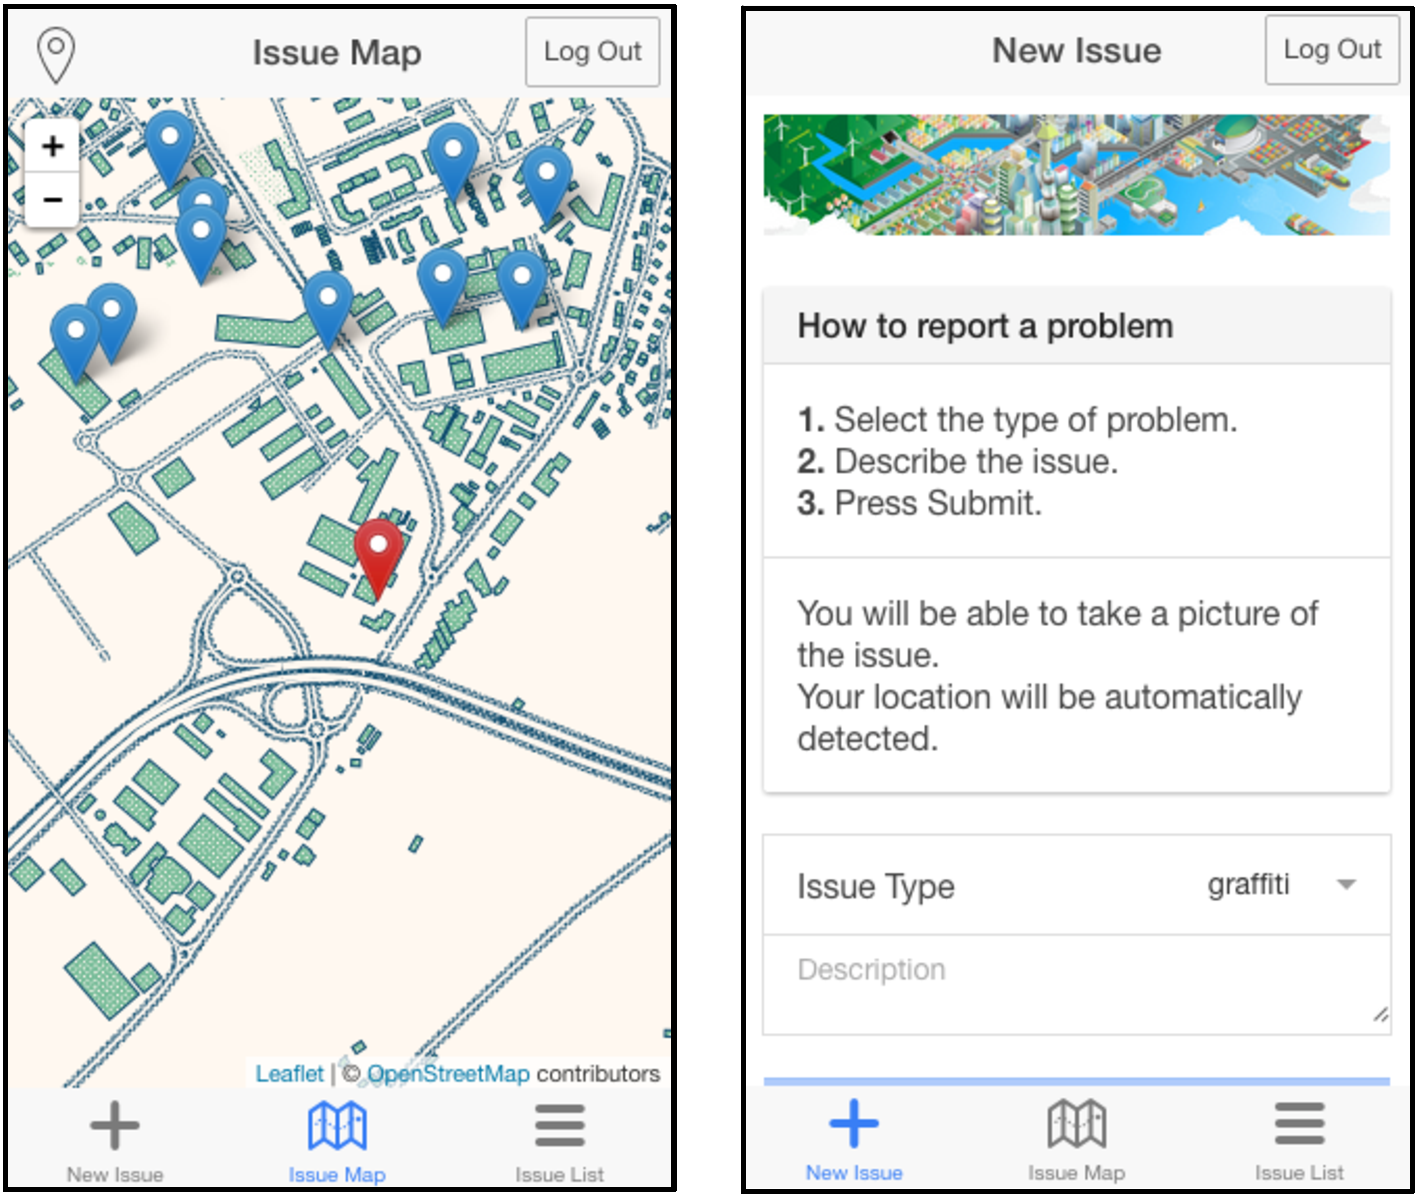
\includegraphics[width=0.8\columnwidth]{figures/citizen-mobile.pdf}
%\caption{The mobile app used to report issues}
%\label{fig:citizenMobile}
%\end{figure}


%\begin{figure}
%\centering
%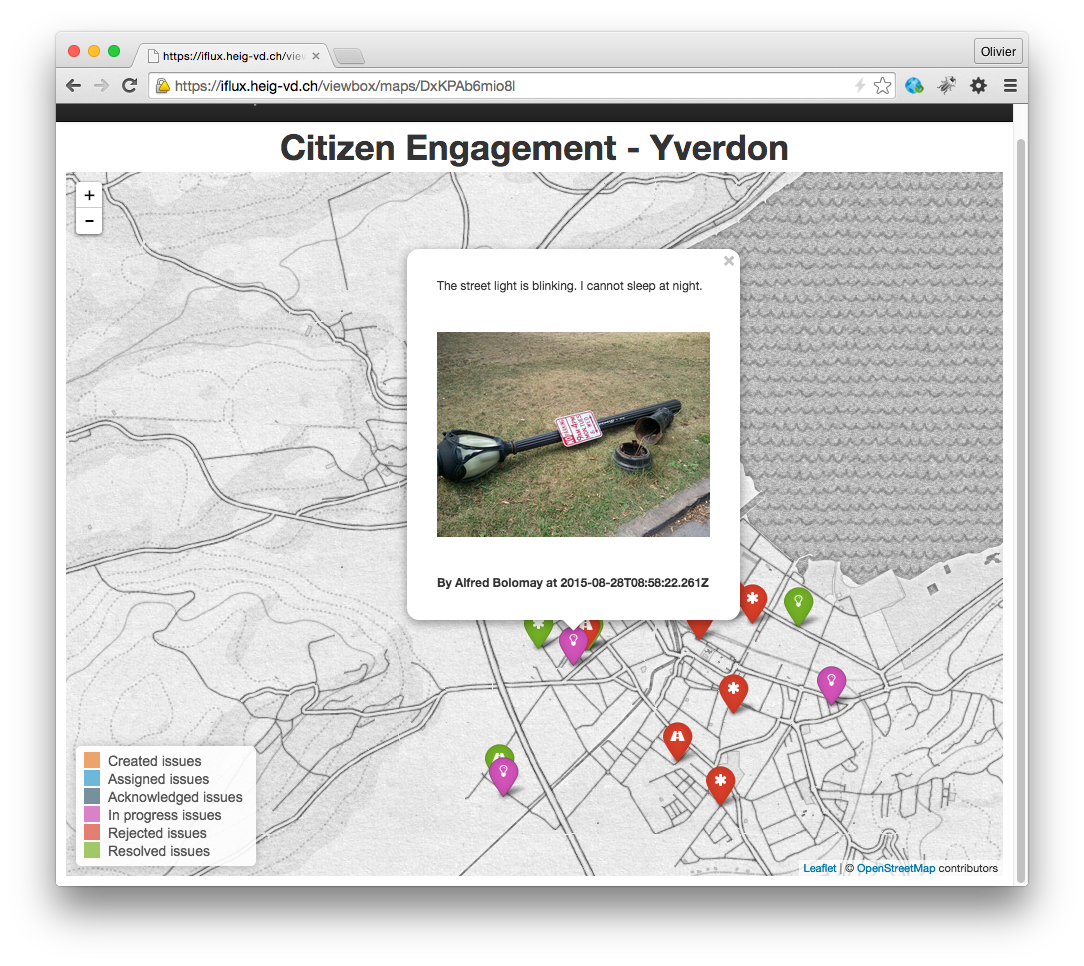
\includegraphics[width=0.9\columnwidth]{figures/citizen-viewbox.png}
%\caption{Issues shown by the ViewBox action target}
%\label{fig:citizenMap}
%\end{figure}

%\begin{figure}
%\centering
%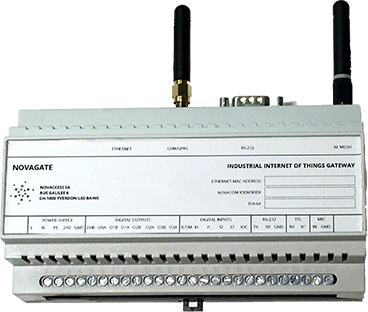
\includegraphics[width=0.8\columnwidth]{figures/novagate.png}
%\caption{The Novaccess IoT gateway is an iFLUX event source}
%\label{fig:novagate}
%\end{figure}


\subsection{Parking @ Paléo}

Paléo Festival is one of the largest music festivals in Switzerland. This year, had the opportunity to evaluate several iNUIT projects in a proof-of-concept deployment. One need expressed by the organizers was to get realtime information about the flow of vehicles and the occupancy of the parkings. To address this question, we created a system composed of one iFLUX \emph{event source} and one iFLUX \emph{action target}. 

The \emph{event source} is a smart object located at the entrance of the parking (see Figure \ref{fig:paleo}), which detects vehicles with ultrasonic sensors. Connected to the Internet via a 802.15.4 mesh network and a WoT gateway, the object emits an event every time a car enters or leaves the parking. The \emph{action target} is responsible for managing application state, which consists of the number of cars currently in the parking, as well as aggregate metrics about the flow of vehicles (number of entries and departures per minute, hour and day). The \emph{action target} publishes this information via a custom REST API, which is used by a web dashboard.

\begin{figure}
\centering
%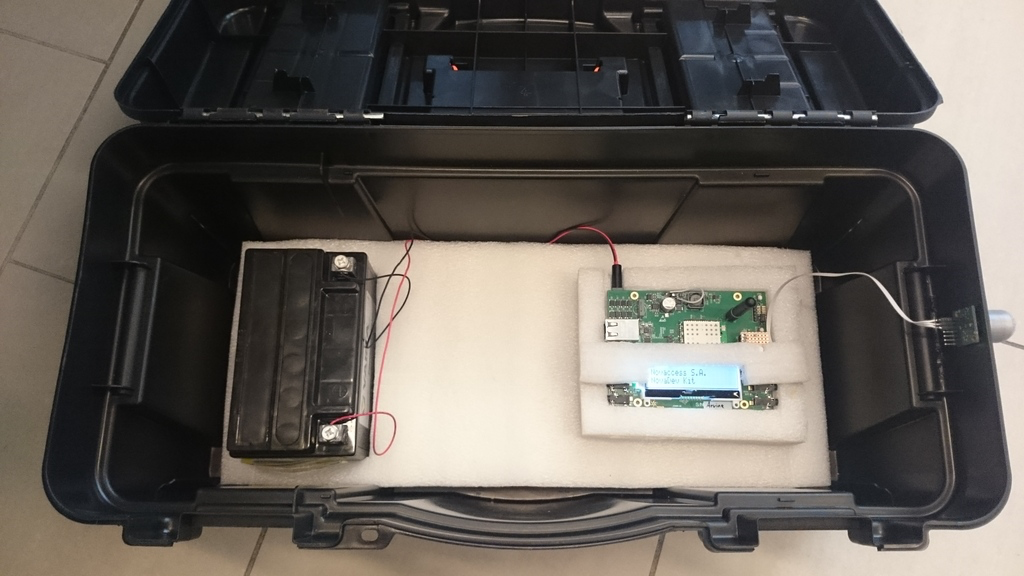
\includegraphics[width=0.9\columnwidth]{figures/paleo-before.png}
%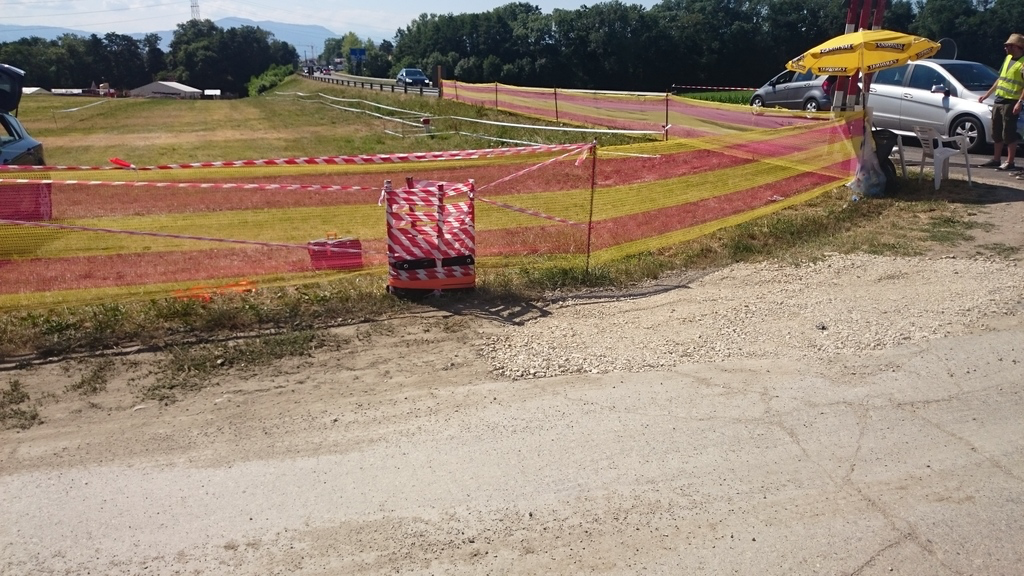
\includegraphics[width=0.9\columnwidth]{figures/paleo-during.png}
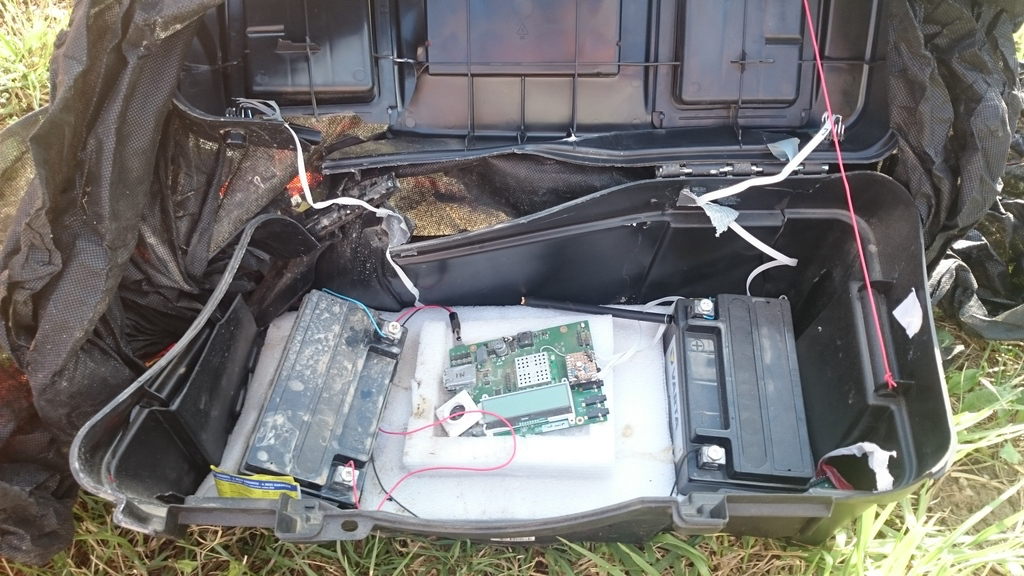
\includegraphics[width=0.85\columnwidth]{figures/paleo-after.png}
\caption{The event source after the festival}
\label{fig:paleo}
\end{figure}


\subsection{Awareness @ Novaccess}

Novaccess is a startup which develops an integrated stack (hardware, firmware, software) for the industrial Internet of Things. Novaccess has developed NovaLight, a smart lighting solution, which allows municipalities to reduce costs by lowering energy consumption and improving maintenance procedures. Measures are collected from street lights (consumption, faults, etc.) and analyzed. The platform can also dynamically and remotely adjust lighting levels.

%\emph{Awareness} is a concept that has been studied extensively in the Computer Supported Cooperative Work (CSCW) literature. While awareness is a somewhat broad concept, with several definitions, we like to think of it as a general sense of what is happening in a particular environment. In the context of Novalight, \emph{awareness} means that the Novaccess team would like to get a better sense about what is happening, on a continuous basis and without effort. The team would like to be able to detect unusual or interesting patterns. There are actually different dimensions that the team would like to be aware of. For example, Novaccess product owners would like to get a sense of the activity of end-users (are they using the web front-end, are they facing issues, are there features that they use a lot, etc.). Also, Novaccess engineers would like to get a sense of the technical activity (are there communication issues, are there faulty components to replace, what is the amount of transmitted commands, etc.).

We have worked with the Novaccess team to develop an \emph{awareness system} with iFLUX, i.e. a system which collects various types of events and generates notifications for the Novaccess staff. Several \emph{event sources} have been created. The first source, embedded in the NovaLight software, emits events that correspond to user actions (e.g. user has logged in, user has sent a command to a street light, etc.) or to technical issues (e.g. the database size has reached a given threshold). The second source, embedded in the NovaLight IoT gateway, emits events that correspond to measures or technical issues. The \emph{action target} used in the system is the Slack gateway presented before. Rules have been configured on the iFLUX middleware to send the text notifications via Slack, when \emph{interesting} events happen. The flexibility of the setup comes from the fact that it is possible to configure more than a rule. This allows the team to fine tune the amount and destination of the generated awareness messages. This simple setup could easily be extended with other notification devices (lava lamps, color LEDs, etc.).


